\documentclass[a4paper,twoside,titlepage]{article}

%--- Packages ----------------------------------------------------------------
\usepackage{a4}
\usepackage[english]{babel}


\usepackage[inner=2cm,top=2cm,outer=3cm,bottom=1cm,includehead,includefoot]{geometry}
\usepackage[latin1]{inputenc}
% \usepackage[utf8]{inputenc}
\usepackage{moreverb}
\usepackage{float}
\usepackage{graphicx}
%\usepackage{makeidx}
%\makeindex
% Don't forget to run makeindex and include \printindex
\usepackage{fancyhdr}
 \usepackage[colorlinks=true,linkcolor=magenta,urlcolor=blue]{hyperref} % Reference by title

\setcounter{tocdepth}{2} % Only subsections in toc

%--- Definitions -------------------------------------------------------------

\def\author			{Group 4}
\def\course			{5DV087 VT10}
\def\coursename	    {Software Engineering}
\def\delivery		{Project Plan}
\def\version		{0.1}
\def\trivialname	{Customer Terminal}
\def\tutor			{}


% New output float
\floatstyle{boxed}
\newfloat{program}{thp}{lop}
\floatname{program}{Program}
\newfloat{output}{thp}{lop}
\floatname{output}{Output}

%\restylefloat{figure}

 \hypersetup{
 pdfauthor = {\author},
 pdftitle = {\trivialname{} - \delivery},
 pdfsubject = {\coursename},
 pdfkeywords = {umu, edu, ruby, plan}
 }


\newcommand{\HUGE}{\fontsize{36}{42}\selectfont{}}
\newcommand{\helvetica}{\fontfamily{phv}\selectfont}
\newcommand{\degree}{\ensuremath{^\circ}}
\pagestyle{fancy}
	\lhead[\coursename]{\today}
	\chead[\textsc{\trivialname~- \delivery}]{\textsc{\trivialname~- \delivery}}
	\rhead[\today]{\course}
	
	\lfoot[\thepage]{\author}
	\cfoot[]{}
	\rfoot[\author]{\thepage}
	
	\renewcommand{\headrulewidth}{0.4pt} 
	\renewcommand{\footrulewidth}{0.4pt}

%-----------------------------------------------------------------------------
\begin{document}
\pagestyle{empty}
%--- Titlepage ---------------------------------------------------------------
\begin{titlepage}
	{
	\helvetica
	\begin{flushright}
		\small \coursename{} \course\\
	\end{flushright}
	\begin{center}
		\LARGE \trivialname\\
		\HUGE { \textbf{\delivery}} \\
		\small \textbf{\author}\\
		\normalsize {
    		Emil Eriksson (c07een)\\
    		Martin �slin (c07man)\\
    		Johan Norberg (c07jng)\\
    		Rickard Westerlund (c07rwd)\\
    		Per Bj�rklund (c07pbd)\\
    		Javid Jou (dv08dju)\\
    		}
		\vspace{95mm}
	\end{center}
	\begin{flushright}
		\subsection*{Assistant}
		Tor Sterner \href{mailto:tors@cs.umu.se}{tors@cs.umu.se}
		\subsection*{Examinator}
		J�rgen B�rstler \href{mailto:jubo@cs.umu.se}{jubo@cs.umu.se}
	\end{flushright}
	}
\end{titlepage}

\pagestyle{fancy}
\pagenumbering{roman}
%--- Table of contents -------------------------------------------------------
\tableofcontents
\clearpage
\newpage

%--- Document ----------------------------------------------------------------
\pagenumbering{arabic}

%-----------------------------------------------------------------------------

\section{Problem description}
For this project the group will design and implement a customer terminal for a large food store. To use the terminal the customer should only have to swipe their customer card and the terminal should display the correct information. The terminal should display general offers, which every customer can use, and special offers, which are unique for the customers that have fulfilled the requirement of the offer. The terminal should also be able to display other information e.g. recipes. The offers themselves can give a percentage discount on the amount or a predefined discount on a specific item. To generate the specific offers the terminal should have a database of some sort which contains information about common and/or regular purchases of the customer that could be compared against the active offers. When the customers is presented with a couple of these offers, they should be able to select and print them, this also applies to other information displayed on the terminal. 
     
For the final presentation of the terminal, where the finished product will be presented for the customer the terminal should be able to run on a regular PC with a external card scanner over an USB interface, also a printer will be attached as the customer should be able to print the selected information. The project should also support a touch screen if this is added later in the project.
 
Other requirement for the usability of the terminal is that the general "look and feel" for the GUI should be similar to ICA's customer terminals and that the terminal would have a very diverse user group so the ease of use is very important. The systems should have a different interface for adding and changing customer data, product data, recipes, etc. This interface should be very simple, as in the real world this would be provided by external systems and therefore a very advanced interface is not needed. Another requirement for the implementation is that should be done using the TDD-method and principles.
    
During the project the group will have to provided the client with a project plan, a report with basic design decisions, GUI mock-up, assumptions, risk management and the time plan for the project, weekly progress reports, reports of what has happened, been done (or not), data on project progress and individual effort, and a final report. The final report should summarize the project, its results (analysis/design, GUI, code), lessons learned and data on individual effort. 
    
The project group is consisting of six members and the time period of the project is six weeks. The purpose of the project is for the group member to practice their skills of working in project teams, project management, a good implementation with a good design and writing reports. 

For more information, see specification \cite{spec}.
	\subsection{Assumptions}
		Some parts of the specification were unclear so an assumption had to be made.
		That both individual offers and general offers will be interpreted the same. The only difference being that there are no conditions that have to be met to be offered the general offers.
	\subsection{Limitations}\label{limitations}
		The operations that the customers will be able to perform at the terminal are limited to the specification and with the specification some limitations will follow.
 
		Blind people will not be able to use the terminal, as the interface is graphical. The terminal could be made with a sound interface but no speakers will be linked to the system according to the specification.

\section{Project management}
	\begin{itemize}
    \item All written reports and presentations will be in English.
    \item For time tracking a spreadsheet in GoogleDocs will be used.
    \item Group meetings every week.
	\end{itemize}

\section{System description}
	\subsection{UML}

		After the preliminary system design was ready a basic UML was created to show the client the structure of the implementation. This UML can be seen in \autoref{fig:uml} on \pagename{} \pageref{fig:uml}.

		Note that this is a preliminary design and could be changed during the course of project. 

	\subsection{Design}

		The architectural design for the project relies on the Model-View-Controller pattern, using a database back end. The back end consists of four different models which handles all the data flows of the system as well as user sessions. These models handles the data for products, customers, offers and recipes.

		The GUI view simply fetches data from the back end as it is requested and displays it. Information such as a welcome to text for the user, available offers and recipes are displayed with the ability to select offers and recipes to be printed out.
		When data is requested to be printed a separate printer view will be used that prints data to be displayed rather than put it on the terminal screen. This data is fetched using controllers that serves as a bridge between the views and models.

	\subsection{Flowchart}

		To show the flow of the program in the terminal a flowchart has been produced, this flowchart shows the way from the card swipe to the printing of the selected offers or recipes. This flowchart can be seen in \autoref{fig:flowchart} on \pagename{} \pageref{fig:flowchart}.

		In the chart all the different actions of the terminal can be seen, these actions are represented as diamonds. All the processes are represented as squares.
   
	\subsection{Tools and Methods}

		The project will be written in Ruby using the Ruby on Rails framework with SQLite as database. Using SQLite will allow for simpler testing as it uses simple files for storage. HTML, CSS and possibly JavaScript will be used for the user interface.
		A specific program for the GUI may therefore not be needed, as any web browser would suffice, using caret browsing mode for full screen viewing and built-in support for touch screen.

		For unit testing we will use Unit::TestCase and measure code coverage with metric\_fu. GIT will be used for revision control of our source code and documents.
		The project will be developed using TDD, and team members with little experience of the tools may need to work in pairs.
\section{GUI}

	In this section we will describe how the system's graphical user interface will look and behave. The user group for this system is very diverse, hence it must be adjusted so it can be used by people that are colorblind, visually impaired or have any other handicap. Since we don't yet know the specifications on the machine that the system will operate on we will try to strive for a GUI that adjust its content dynamically depending on resolution. 

	The only form of user input to the GUI will also be done via buttons, mostly for navigation and browsing along with a few commands such as print and log out. To gain access to the machine the user will have to swipe their ICA membership card. 
	
	The mock-ups for the GUI are available in \figurename{} \ref{fig:gui_login}, \ref{fig:gui_welcome}, \ref{fig:gui_offers} and \ref{fig:gui_recipe}.

	\subsection{Accessibility}
		We will strive to make the overall system very easy to use and always have help available, either as pictured tutorials, help text or an easy way to contact support staff on location. 

		\subsubsection{Colorblindness}
			Around 8\% of males and 1\% of females suffer from colorblindness of different degree, therefore we will strive for a system that does not rely on colors at all to communicate with the user. There are even people that can only see shades of gray, hence why no reliance on colors is used. Even if we tried to adjust it to fit one group of colorblind people, it would not work on another group.

 			Since the system is very basic to begin with this will not be a difficult task to accomplish and the main focus will be to distinguish buttons from the background. A button should look like a raised button and not just a text label.

		\subsubsection{Simplicity}
			Since some of the users might not have a lot of experience with interactive systems we will strive for a very simplistic GUI design. It should not possible for the user to misunderstand or misinterpret the actions he/she is able to perform, or understand the data presented.

		\subsubsection{Visual impairment}
			The system will strive to be usable by most of the visually impaired population except blind people as stated in \autoref{limitations}.

			In order to achieve this all buttons, text and labels will be much larger then normal. This can easily be achieved without making the GUI ``messy'' since we have very few buttons in a big area. Any exact values cannot be given before we receive the exact specifications for the machine. 

\section{Schedule}
	We have devised a schedule that can be viewed in \autoref{fig:schedule} on \pagename{} \pageref{fig:schedule}.  The tasks in the schedule have been set up in a way so that they both work as milestones and tasks. All of which derives from functionally in the system. The schedule also specifies how much time we plan to spend on each task. A total of 570 hours have been planned for the different tasks, out of a total of 672 hours available. Which means we have a buffer of 102 hours. This time can be used for unidentified problems that might occur during the life of the project.

\section{Quality Assurance}
	The following sections will discuss the different quality goals, risks and areas of responsibility. 
	\subsection{Quality Goals}
		To ensure the quality of the implementation the TDD-method and principles are apply to the development of the program. Some of the metrics that will be checked regularly are listed below.

	\subsection{Intuitive interface for a diverse customer base}
	\begin{itemize}
	 	\item A code coverage of at least 90\%
		\item An LCOM (defined by Henderson-Sellers) of no more than 0.6.
		\item Fan-In and Fan-Out values of no more than 5
		\item Satisfy all the requirements in the specification
	\end{itemize}

	\subsection{Risks}
		During a project many things can go wrong, some of these things was notice during the planing phase of the project. What this
		\begin{description}
        	\item[Little time with scanner]
			Since we are five groups with only one scanner it will give us very little time to test our system with it. This could lead to our system not being completely functional with the scanner. We will try to mitigate this by carefully scheduling time with the scanner.
        	\item[Little time with touchscreen]
			As the touchscreen has been ordered but the arrival date is unknown we might get a very limited time to test our system with the touchscreen.
			To mitigate this we will try to have our system working with a mouse. This way there should be no need to test our system with the touch screen. Because most systems does distinguish between input from a mouse or a touchscreen. 
        	\item[Touch screen might not show up]
			If the touch screen never arrives because of some problems with delivery or availability, we won't be able to present our final product. To avoid this happening we will try to have the product also working with a regular mouse pointer so that we can present our system that way.
        	\item[Loss of team members]
			Since there are six members in the team there is a high chance that one or more members will become unavailable because of sickness or due to some other circumstance. This could lead to loss of competence in for example SQL that only a few members know. It can also lead to loss of knowledge in our own system. To mitigate this the members will have to inform the rest of the team as fast as possible so that they can decide what to do. Also the members will inform the group of what they are working with and how the parts they have developed works. This way there should be no real loss knowledge of the system.
        	\item[Conflicts]
			In larger groups there might be many different ideas which can lead to conflicts within the group.This will be mitigated by having lots of meetings where all the ideas are discussed thoroughly until a agreement is reached and if no agreement is met then a there will be a vote on which idea to use.
		\item[Misinterpreted specification]
			If the specification is misinterpreted it could lead to a system that does not meet all the customers requirements. This will be mitigated by asking costumer whenever a requirement is unclear.
		\item[Lack of experience with development tools]
			Most of the group are inexperienced with the tools that will be used to develop the software. Such as, Rails, Ruby, HTML, CSS-templates, JavaScript and SQL. This could lead to the project taking more time than if we were experienced, it also puts more pressure on the team members with the knowledge of the tools.
			We will try to mitigate this by having the team members study up on the parts that they are inexperienced with so that we all can contribute.
		\item[Testing GUI for a diverse customer base]
			Since we have limited time on the project it will be hard to have an extensive testing phase where a very diverse group of people will test the system. This could lead to the GUI not being user friendly for all intended customers. We will try to mitigate this by carefully analyzing which people could be using the system and from there develop a GUI that they all could feel comfortable using.
		\end{description}

% section introduction (end)

% \clearpage
% \appendix
% \newpage
% \section{Source code} % (fold)
% \label{sec:source_code}

% section source_code (end)


%referenslista
 \bibliographystyle{plain}
 \bibliography{plan}

    %%%%%%%%%%%%%%%% bilagor %%%%%%%%%%%%%%%%
    \clearpage
    \appendix

            \begin{figure}[ht]
               \centering
                  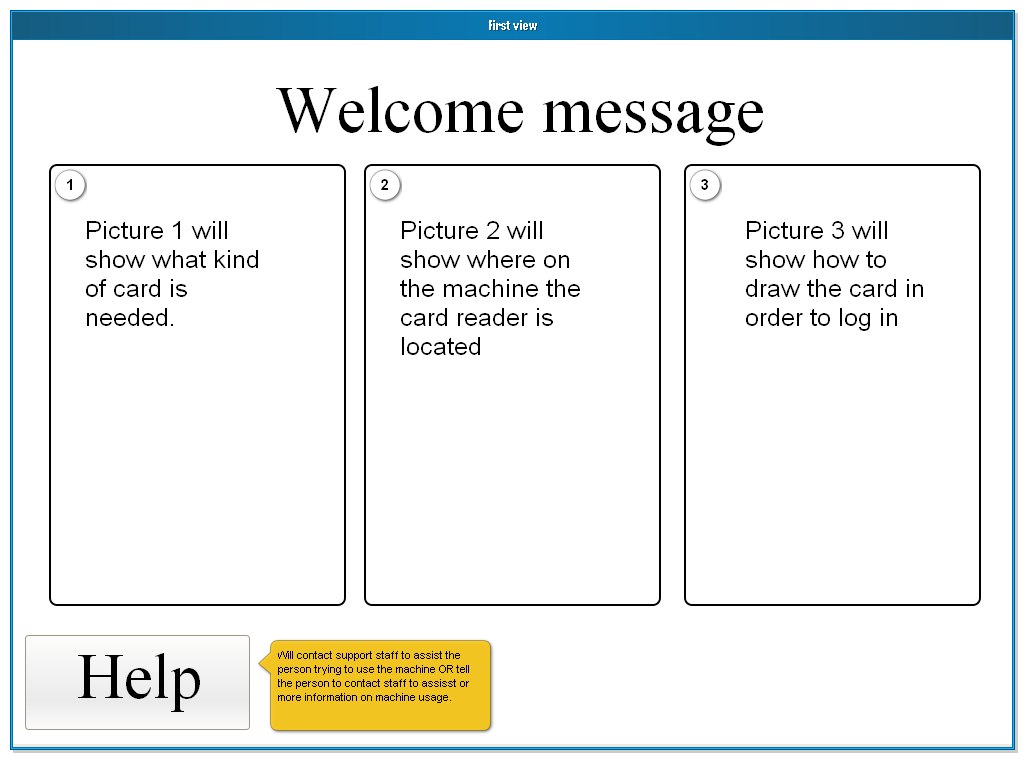
\includegraphics[scale=.3]{images/gui/ica1.png}
               \caption{The first screen the user is greeted with}
               \label{fig:gui_login}
            \end{figure}

            \begin{figure}[ht]
               \centering
                  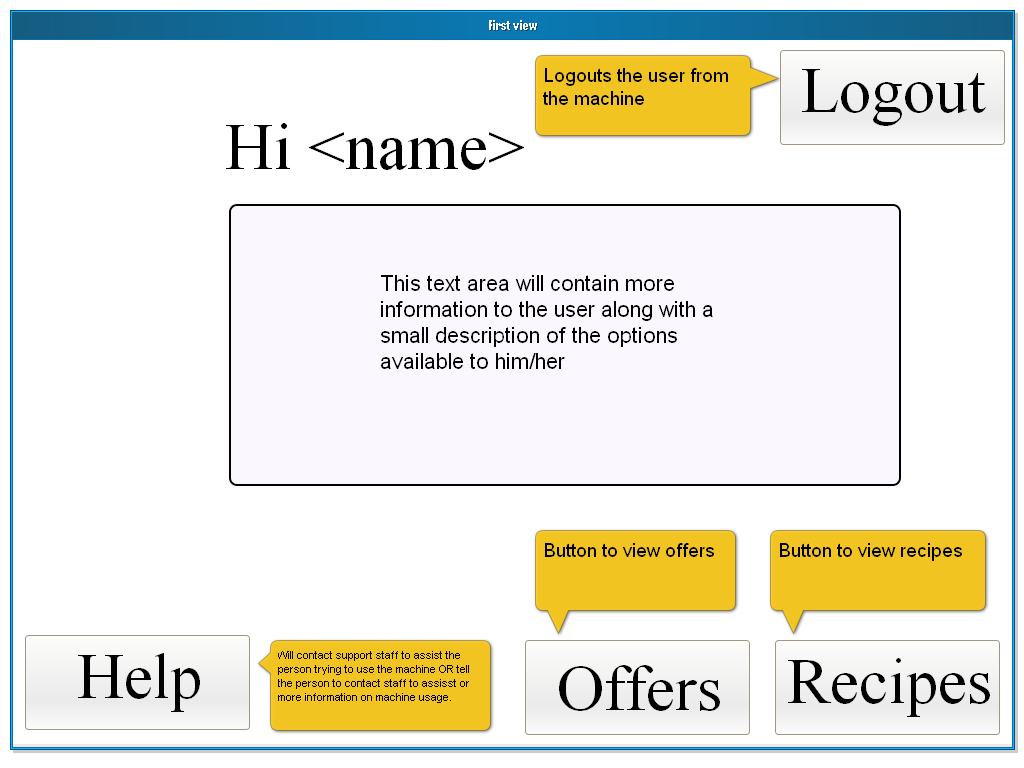
\includegraphics[scale=.3]{images/gui/ica2.png}
               \caption{The "Welcome" screen}
               \label{fig:gui_welcome}
            \end{figure}

            \begin{figure}[ht]
               \centering
                  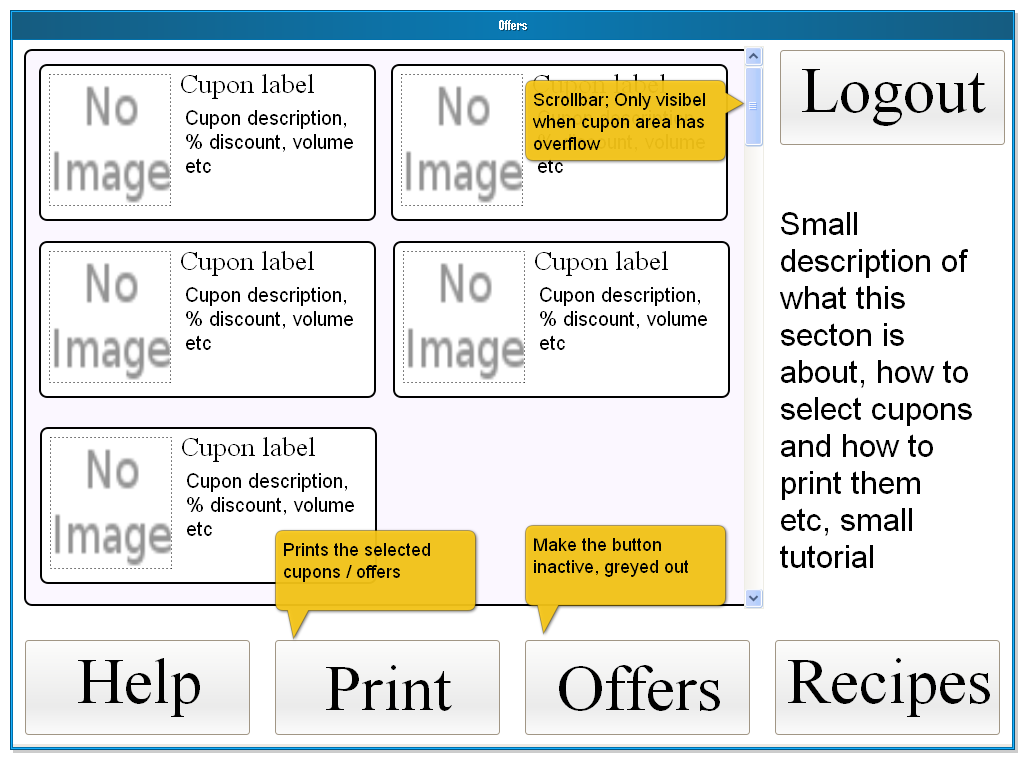
\includegraphics[scale=.3]{images/gui/icaoffers.png}
               \caption{The view of offers}
               \label{fig:gui_offers}
            \end{figure}

            \begin{figure}[ht]
               \centering
                  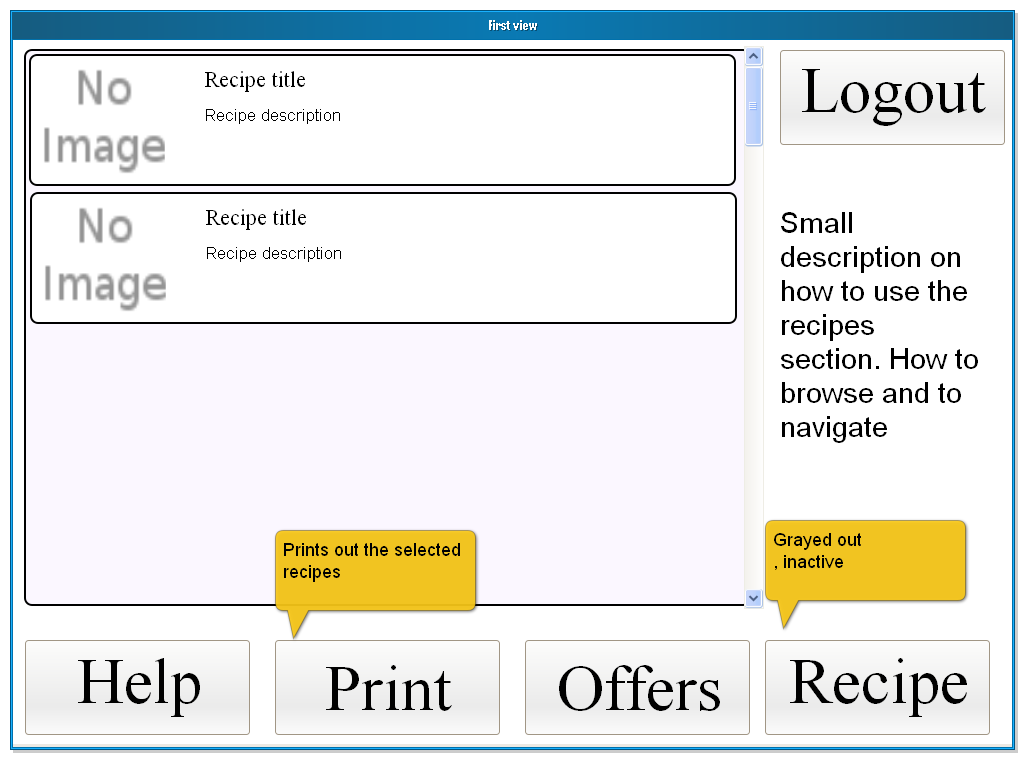
\includegraphics[scale=.3]{images/gui/icarecipe.png}
               \caption{The view of recipe}
               \label{fig:gui_recipe}
            \end{figure}

             \begin{figure}[htp]
                 \centering
                 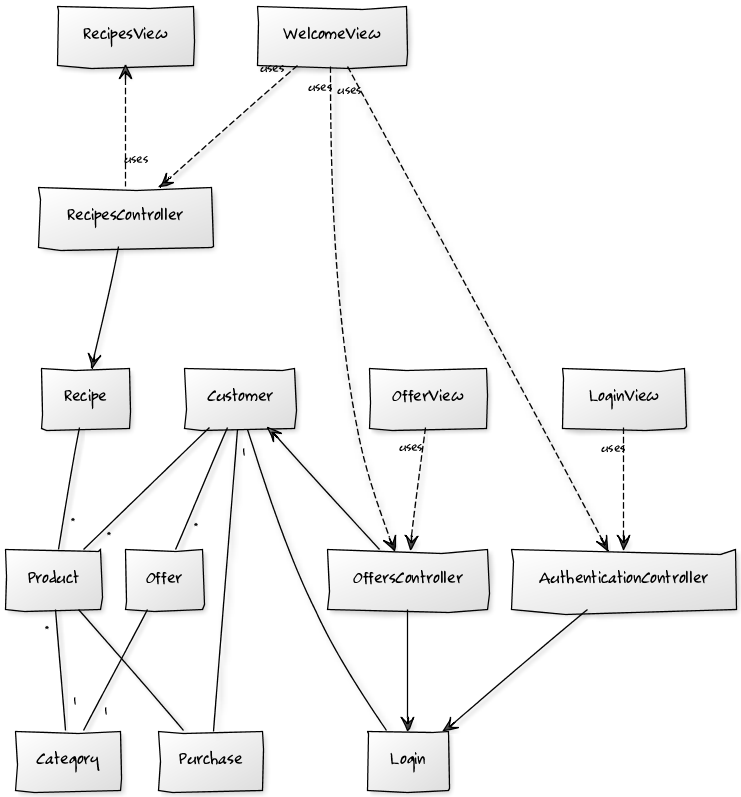
\includegraphics[scale=.83]{./images/uml.png}
                 \caption{An initial UML class diagram.}
                 \label{fig:uml}
             \end{figure}

             \begin{figure}[htp]
                 \centering
                 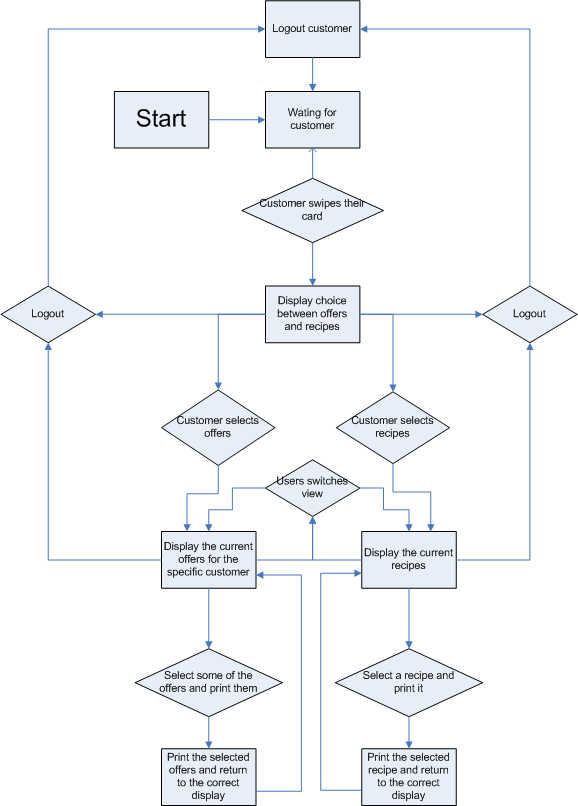
\includegraphics[scale=.5]{./images/flowchart.png}
                 \caption{A flow chart describing the system.}
                 \label{fig:flowchart}
             \end{figure}

             \begin{figure}[htp]
                 \centering
                 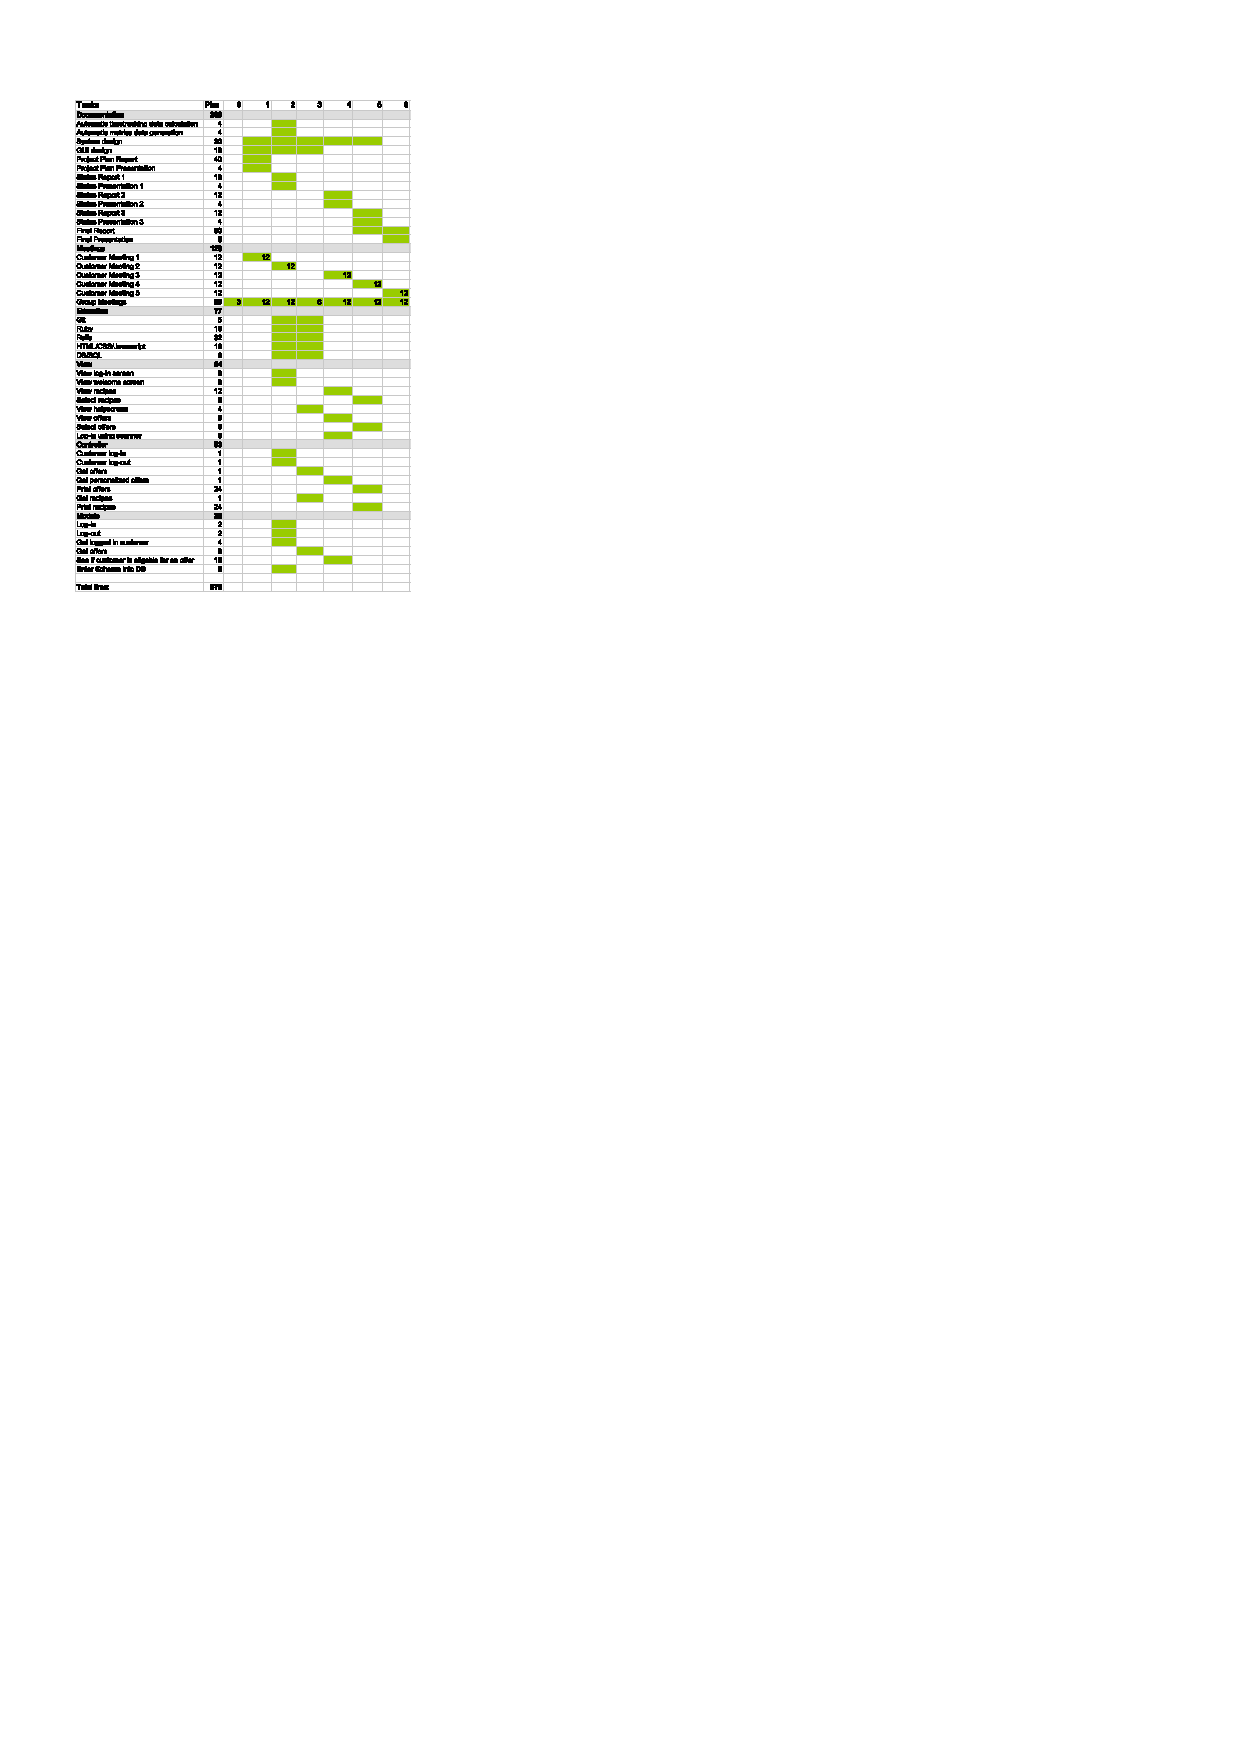
\includegraphics[scale=2]{./images/schedule.pdf}
                 \caption{A flow chart describing the system.}
                 \label{fig:schedule}
             \end{figure}
\end{document}
